% !TeX spellcheck = en_GB

\section{Mean error and mean absolute error}%\hfill} 
\label{app:mean_error}

%%% image bias %%%%%%%%%%%%%%%%%%%%%%%%%%%%%%%%%%%%%
\begin{figure}[h]%\ContinuedFloat
		\centering
        % pres
		\begin{subfigure}[b]{0.49\textwidth}
			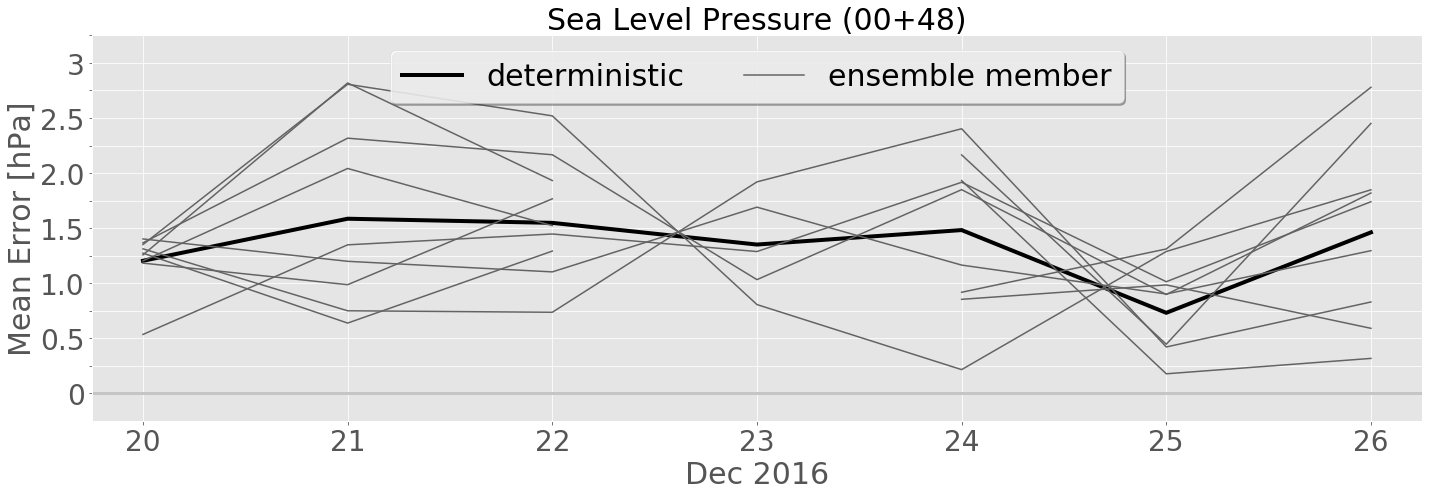
\includegraphics[width=\textwidth]{./fig_sfc_pressure/ME_20161220_26_00}
			\caption{}\label{fig:bias:pres}
		\end{subfigure}
        \begin{subfigure}[b]{0.49\textwidth}
			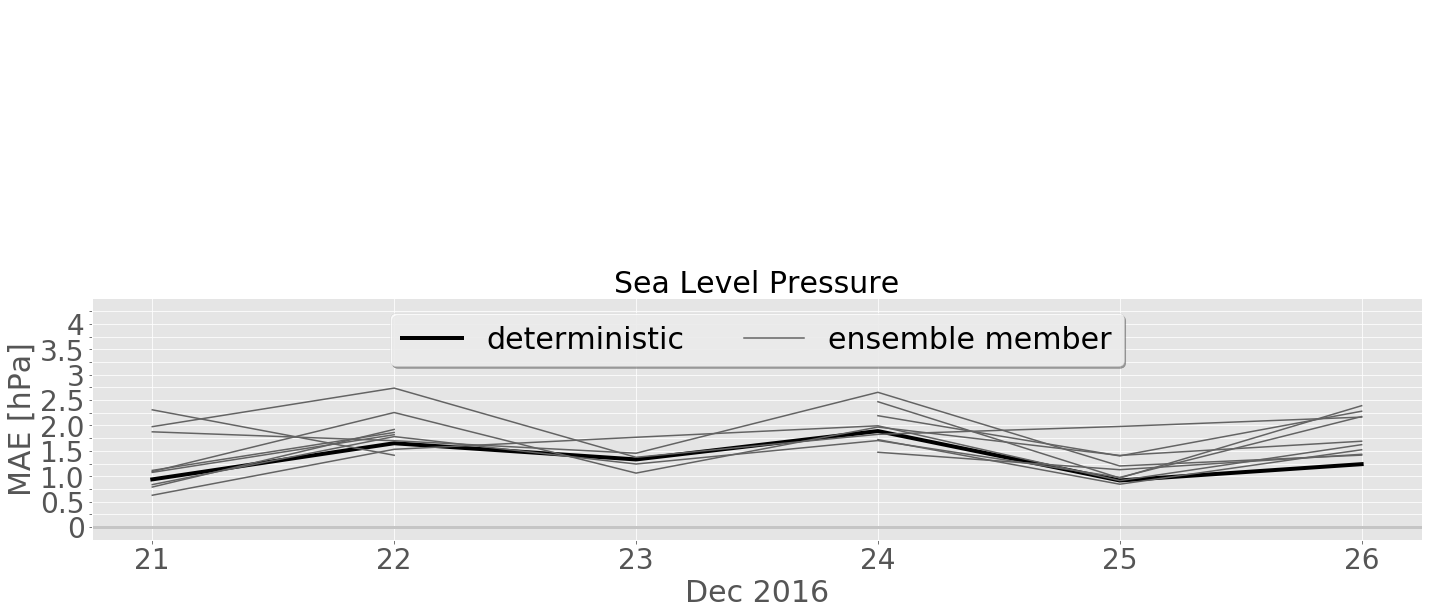
\includegraphics[width=\textwidth]{./fig_sfc_pressure/MAE_20161220_26_00}
			\caption{}\label{fig:MAE:pres}
		\end{subfigure}
		% temp
		\begin{subfigure}[b]{0.49\textwidth}
			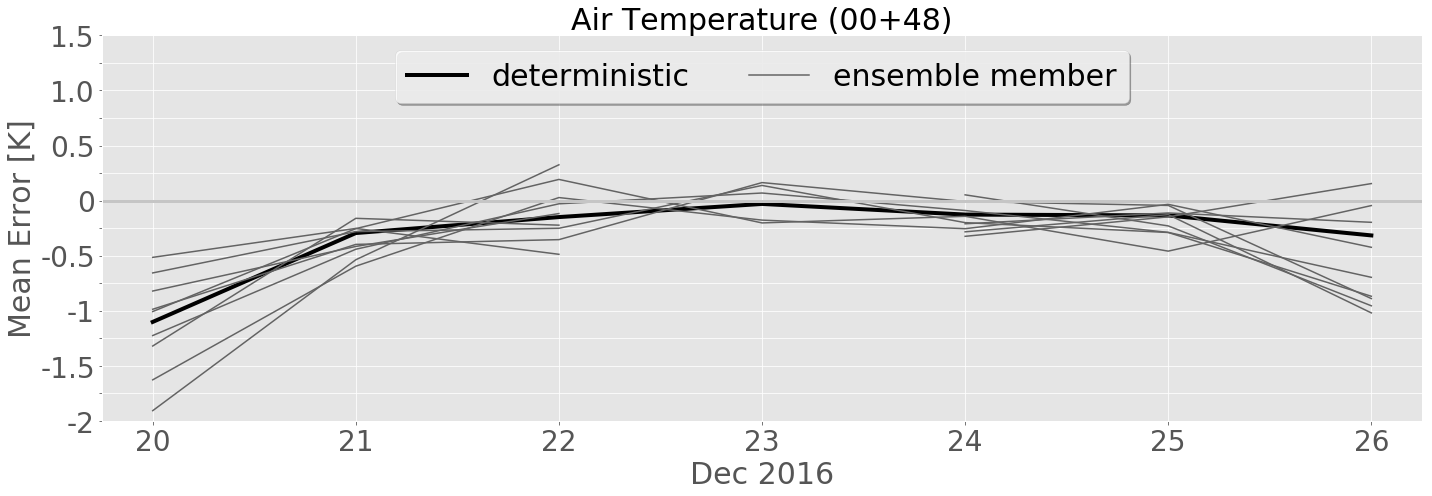
\includegraphics[width=\textwidth]{./fig_sfc_temp/ME_20161220_26_00}
			\caption{}\label{fig:bias:temp}
		\end{subfigure}
        \begin{subfigure}[b]{0.49\textwidth}
			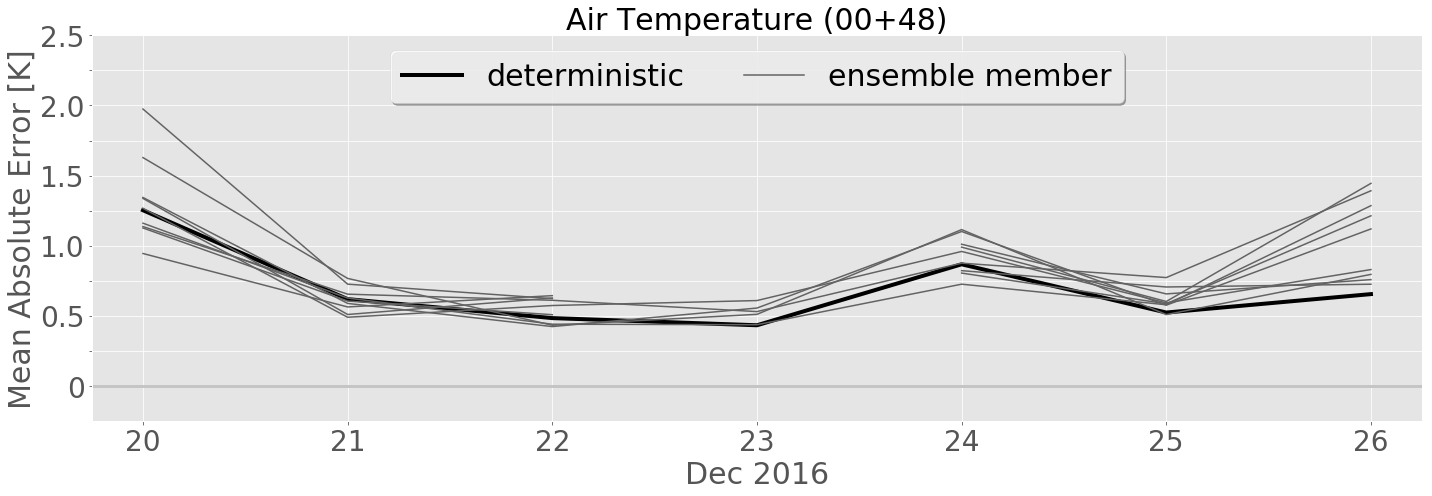
\includegraphics[width=\textwidth]{./fig_sfc_temp/MAE_20161220_26_00}
			\caption{}\label{fig:MAE:temp}
		\end{subfigure}
        % wd
		\begin{subfigure}[b]{0.49\textwidth}
			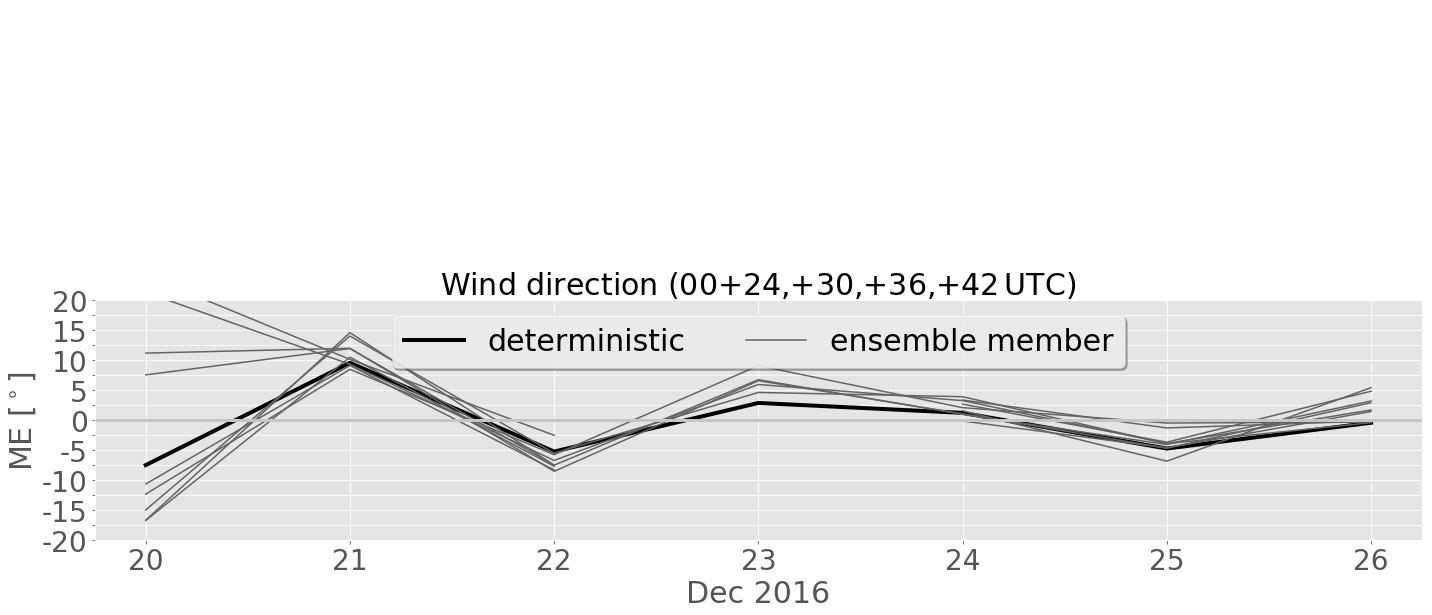
\includegraphics[width=\textwidth]{./fig_sfc_wd/ME_20161220_26_00}
			\caption{}\label{fig:bias:wd}
		\end{subfigure}
        \begin{subfigure}[b]{0.49\textwidth}
			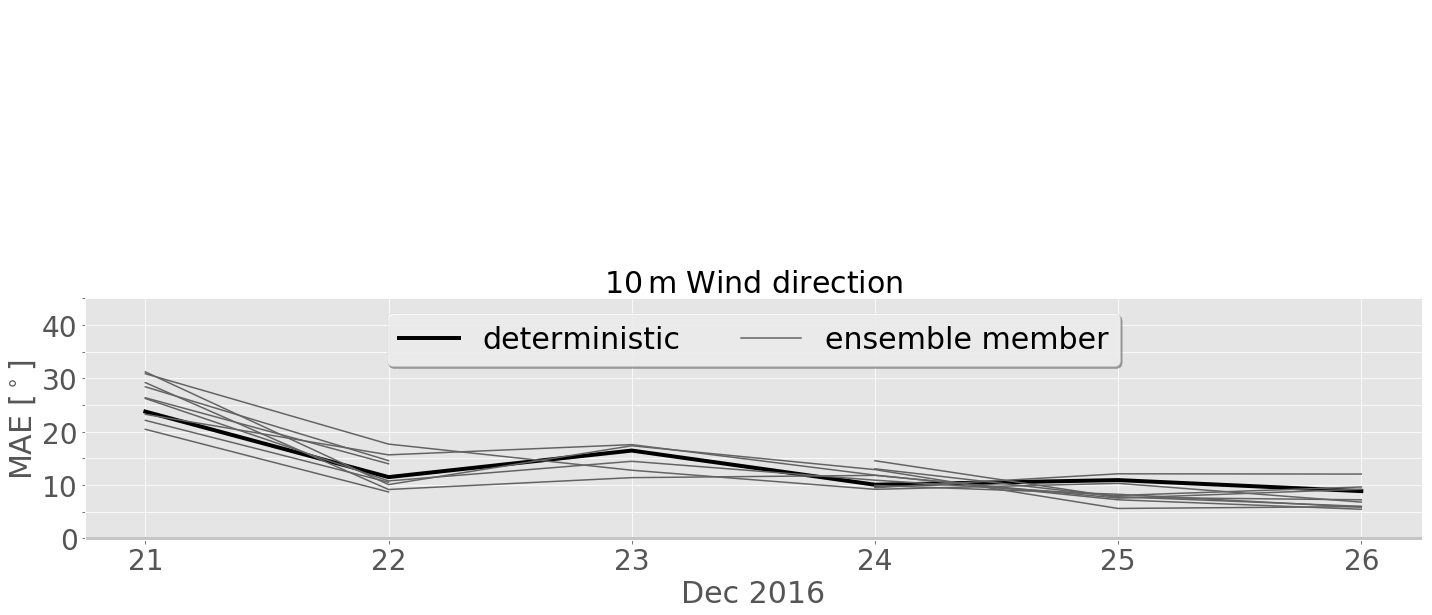
\includegraphics[width=\textwidth]{./fig_sfc_wd/MAE_20161220_26_00}
			\caption{}\label{fig:MAE:wd}
		\end{subfigure}
\caption{Mean error (\protect\subref{fig:bias:pres}, \protect\subref{fig:bias:temp}, \protect\subref{fig:bias:wd}, \protect\subref{fig:bias:ws}, \protect\subref{fig:bias:precip}) and mean absolute error (\protect\subref{fig:MAE:pres}, \protect\subref{fig:MAE:temp}, \protect\subref{fig:MAE:wd}, \protect\subref{fig:MAE:ws}, \protect\subref{fig:MAE:precip}) of surface variables for all ten ensemble members at Haukeliseter, initialisations at \SI{0}{\UTC}, valid for \SI{48}{\hour}. From top to bottom, sea level pressure (\protect\subref{fig:bias:pres}, \protect\subref{fig:MAE:pres}), \SI{2}{\metre} air temperature (\protect\subref{fig:bias:temp}, \protect\subref{fig:MAE:temp}), \SI{10}{\metre} wind direction (\protect\subref{fig:bias:wd}, \protect\subref{fig:MAE:wd}).}\label{fig:bias_MAE}
\end{figure}
\begin{figure}\ContinuedFloat
	\centering
		% ws
		\begin{subfigure}[b]{0.49\textwidth}
			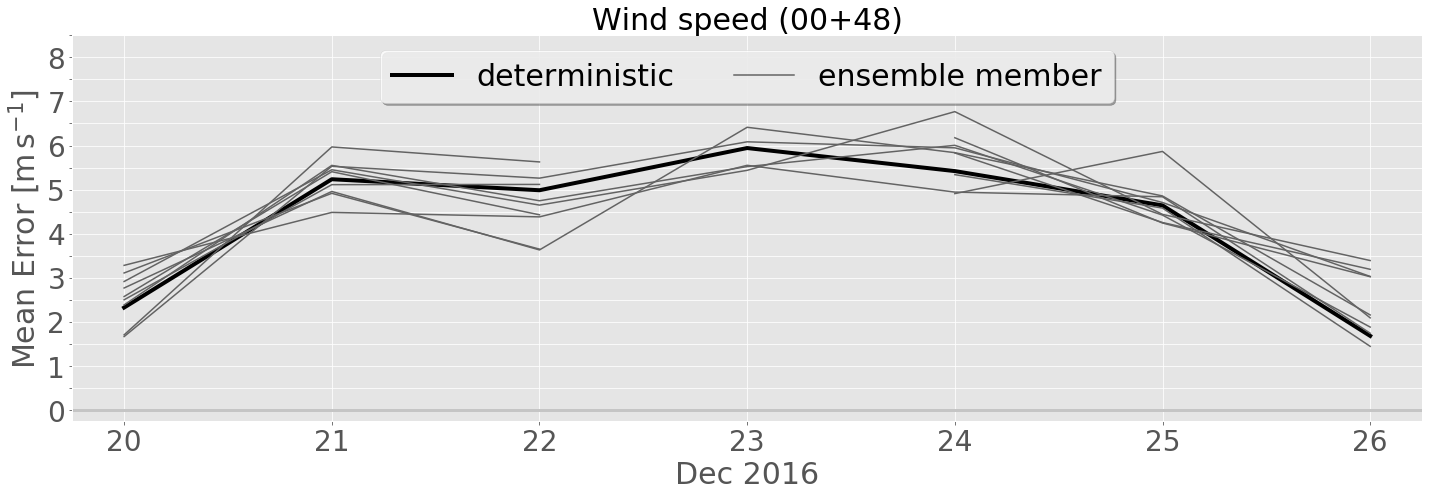
\includegraphics[width=\textwidth]{./fig_sfc_ws/ME_20161220_26_00}
			\caption{}\label{fig:bias:ws}
		\end{subfigure}
        \begin{subfigure}[b]{0.49\textwidth}
			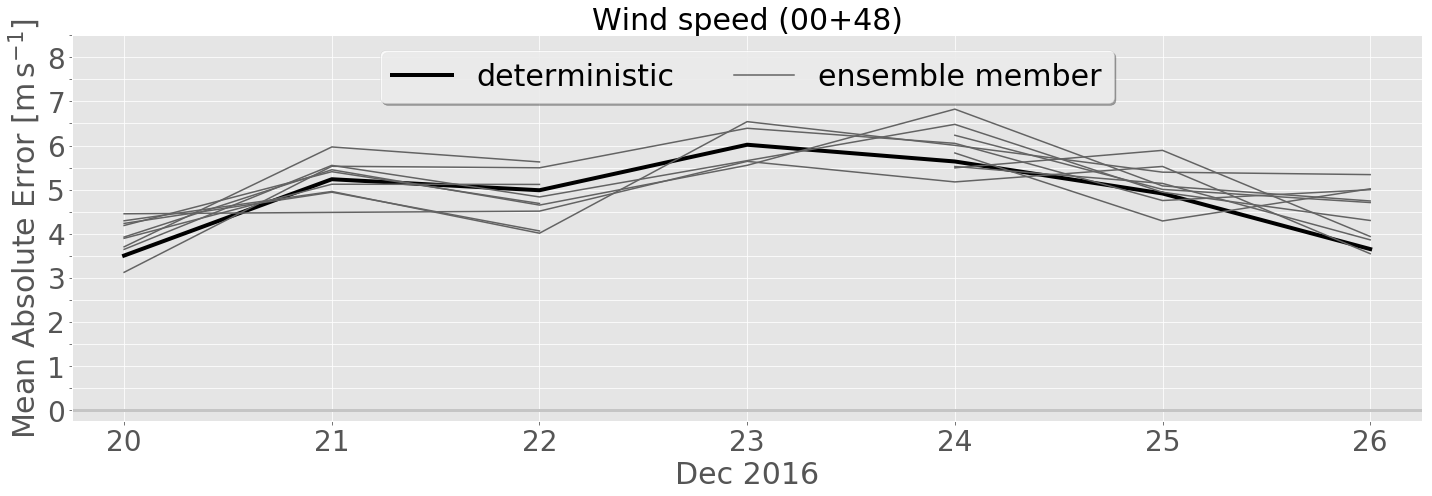
\includegraphics[width=\textwidth]{./fig_sfc_ws/MAE_20161220_26_00}
			\caption{}\label{fig:MAE:ws}
		\end{subfigure}
% \end{figure}
% \begin{figure}\ContinuedFloat
% \centering
        % precip
		\begin{subfigure}[b]{0.49\textwidth}
			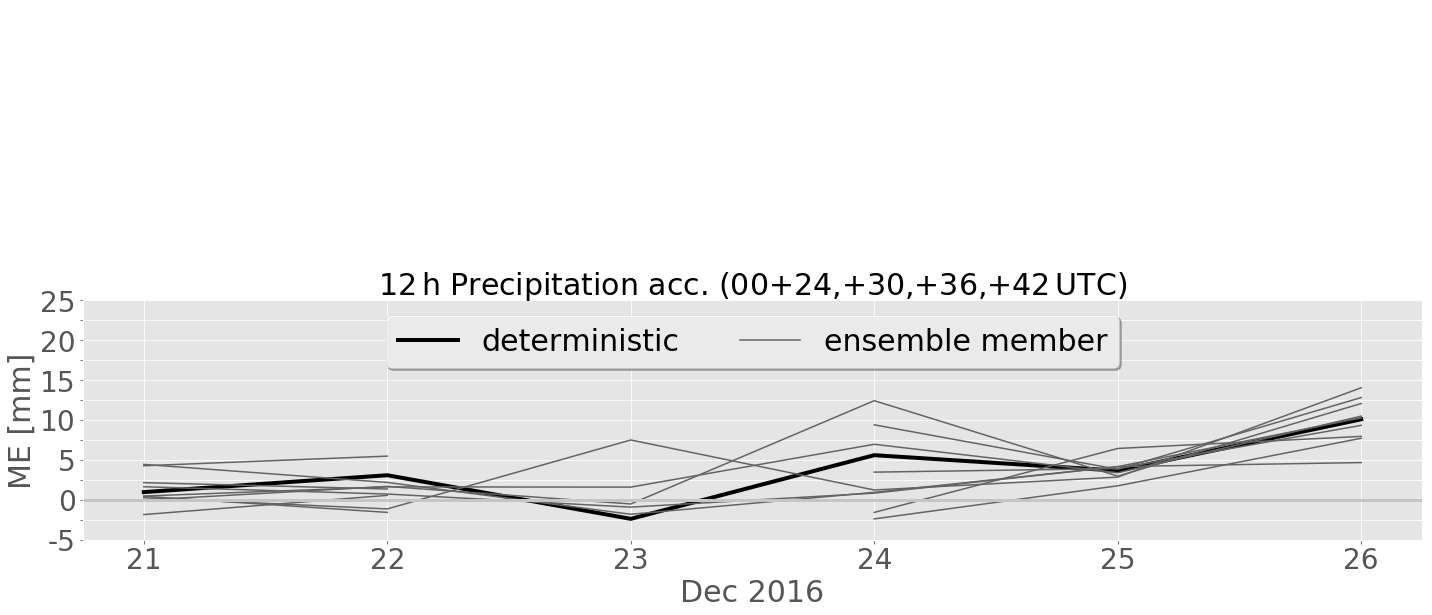
\includegraphics[width=\textwidth]{./fig_sfc_precip/ME_20161220_26_00}
			\caption{}\label{fig:bias:precip}
		\end{subfigure}
        \begin{subfigure}[b]{0.49\textwidth}
			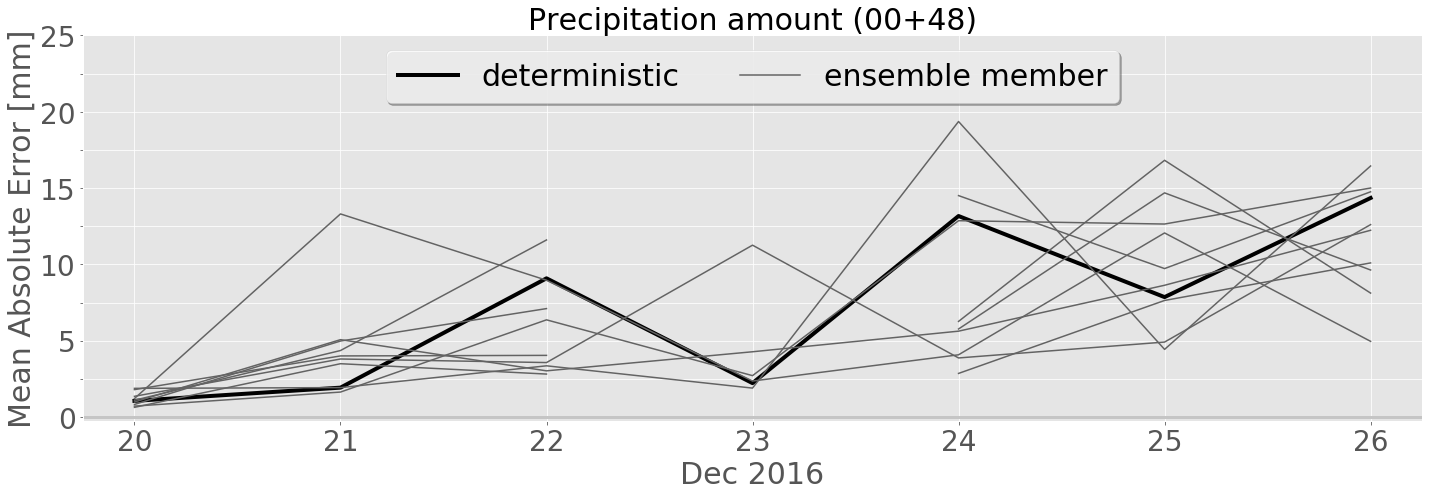
\includegraphics[width=\textwidth]{./fig_sfc_precip/MAE_20161220_26_00}
			\caption{}\label{fig:MAE:precip}
		\end{subfigure}
        % precip 12h
        \begin{subfigure}[b]{0.49\textwidth}
			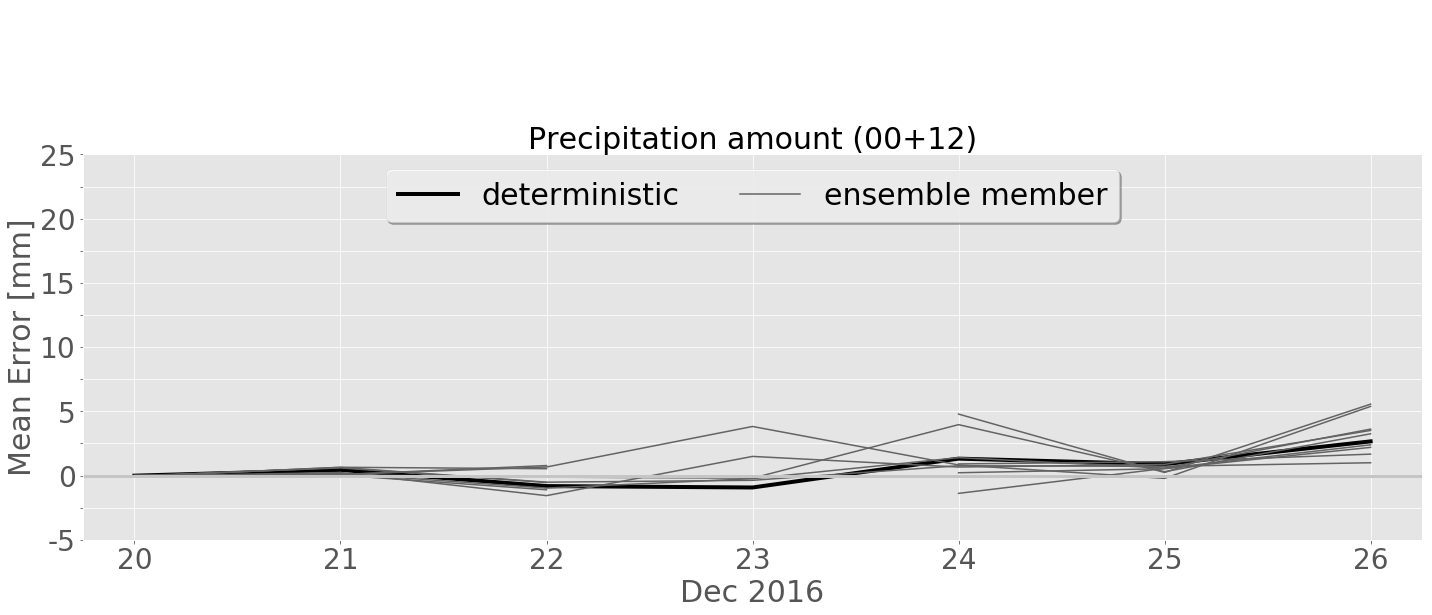
\includegraphics[width=\textwidth]{./fig_sfc_precip/ME12_20161220_26_00}
			\caption{}\label{fig:bias:precip12}
		\end{subfigure}
        \begin{subfigure}[b]{0.49\textwidth}
			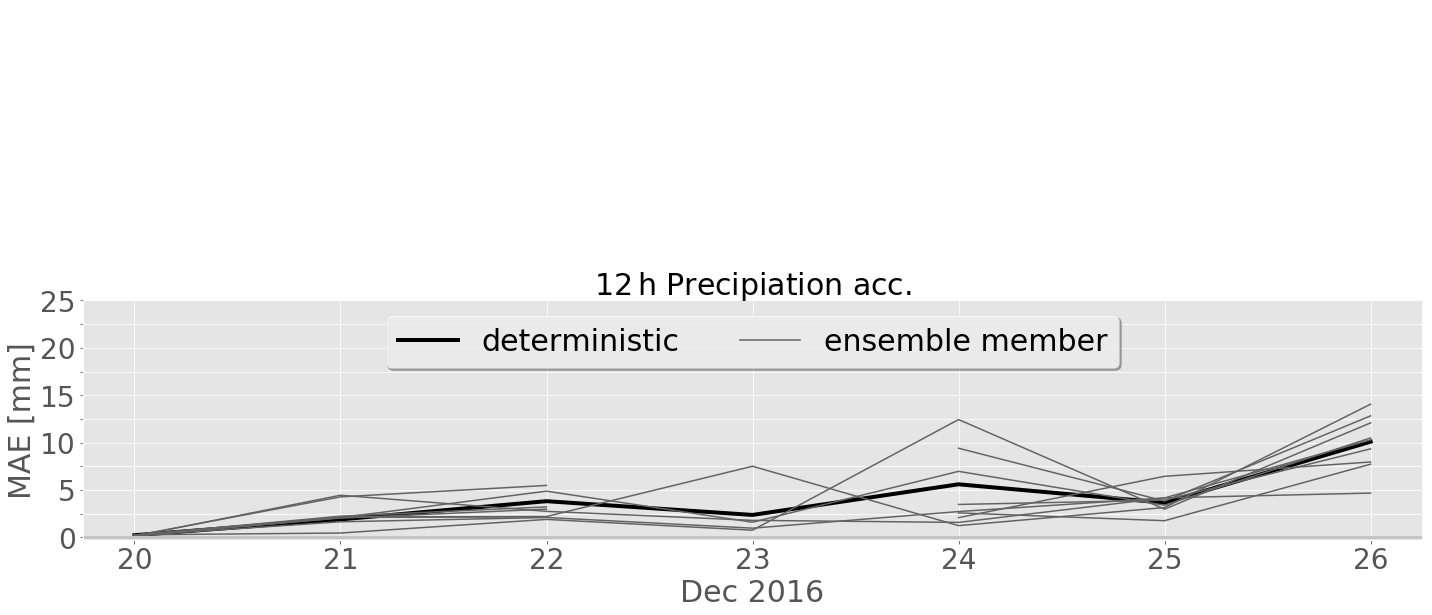
\includegraphics[width=\textwidth]{./fig_sfc_precip/MAE12_20161220_26_00}
			\caption{}\label{fig:MAE:precip12}
		\end{subfigure}
	\caption{\textit{(Continued from previous page.)} ,  \SI{10}{\metre} wind speed (\protect\subref{fig:bias:ws}, \protect\subref{fig:MAE:ws}), precipitation accumulation for \SI{48}{\hour} (\protect\subref{fig:bias:precip}, \protect\subref{fig:MAE:precip}) and \SI{12}{\hour} surface accumulation (\protect\subref{fig:bias:precip12}, \protect\subref{fig:MAE:precip12}). }    
\end{figure}
%%%%%%%%%%%%%%%%%%%%%%%%%%%%%%%%%%%%%%%%%%%%%%%%%%%%%%%%%%%%%%%%%%%%%%%%%%
